\begin{frame}
  \frametitle{Choropleth}/Users/ravahere/Documents/S5_M1MIND/MIND_S2/wwstatviz/beamer/src/demo.tex

  \begin{lstlisting}[language=Python,numbers=left]
  v = Visualizer('path/to/file.csv')
  fig = v.choropleth(title = '...',
                  features = 'all',
                  countries = 'all')
  fig.show() # for inline display (in browsers for example)
  \end{lstlisting}

  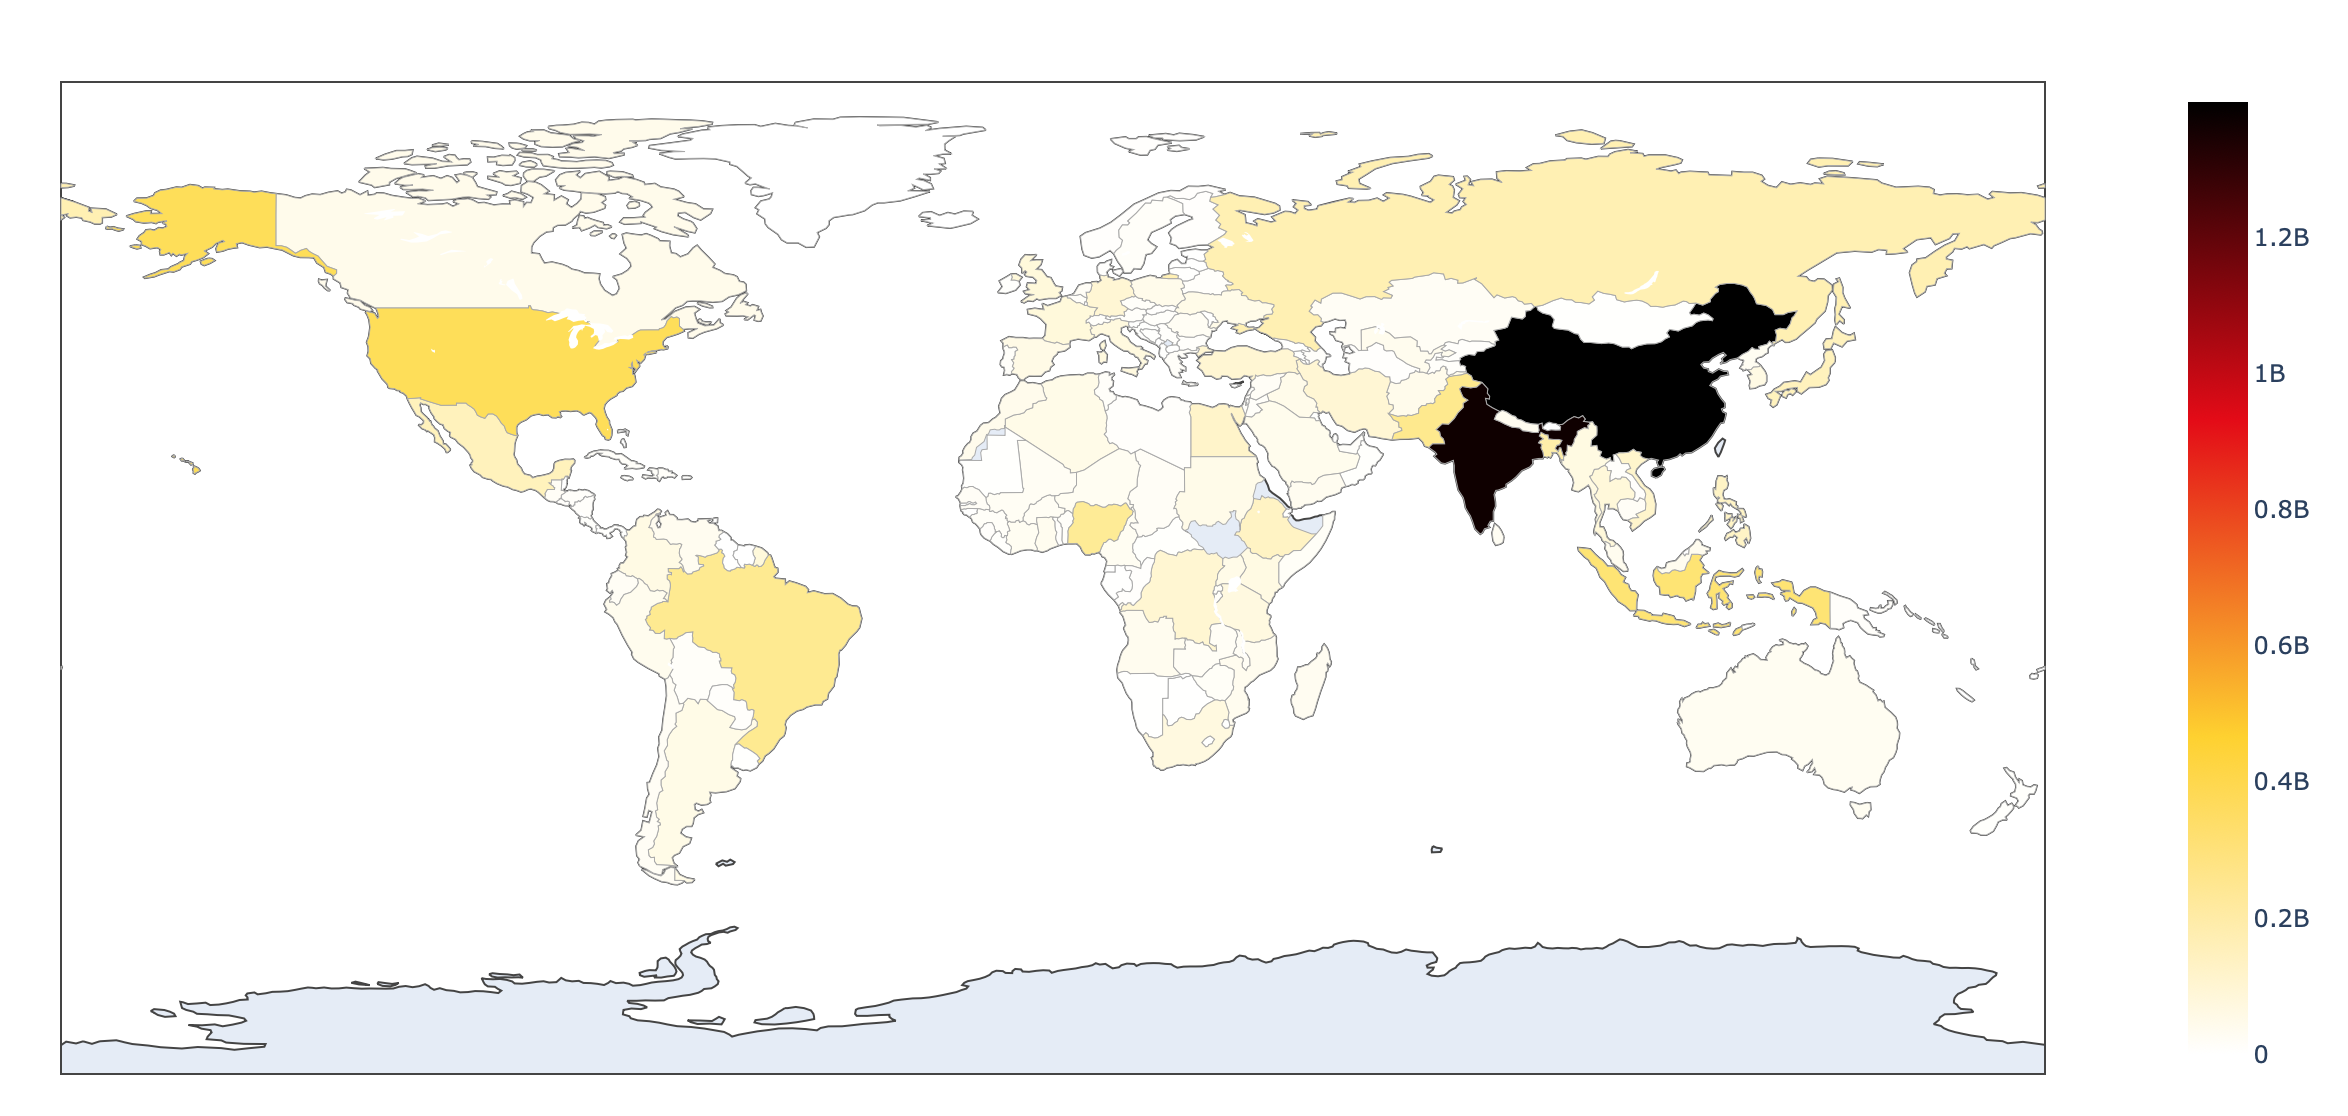
\includegraphics[scale=0.4]{../inc/graphics/choropleth.png}
  
\end{frame}

\begin{frame}
  \frametitle{Heatmap}

  \begin{lstlisting}[language=Python,numbers=left]
  v = Visualizer('path/to/file.csv')
  fig = v.heatmap(countries='all', features='all',
                  method='pearson', mask=True,
                  title='', xlabel='', ylabel='')
  fig.show() # for inline display (in browsers for example)
  \end{lstlisting}
  
  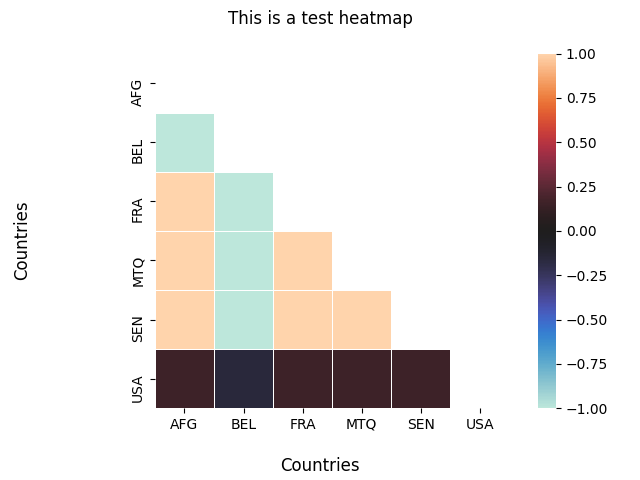
\includegraphics[scale=0.4]{../inc/graphics/heatmap.png}

\end{frame}

\begin{frame}
  \frametitle{Time Series Plot}

  \begin{lstlisting}[language=Python,numbers=left]
  v = Visualizer('path/to/file.csv')
  fig = v.line(countries='all', features='all',
              title='', xlabel='', ylabel='', 
              legend=False)
  fig.show() # for inline display (in browsers for example)
  \end{lstlisting}
  
  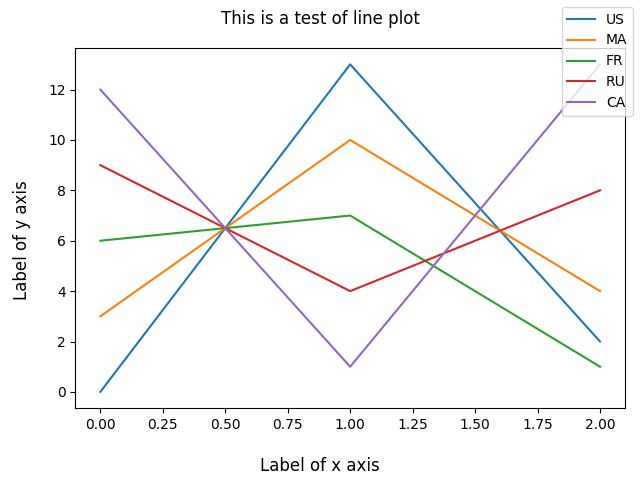
\includegraphics[scale=0.4]{../inc/graphics/line.png}

\end{frame}

\begin{frame}
  \frametitle{Histogram}

  \begin{lstlisting}[language=Python,numbers=left]
  v = Visualizer('path/to/file.csv')
  fig = v.histogram(countries='all', features='all',
                    title='', xlabel='', ylabel='', 
                    legend=False)
  fig.show() # for inline display (in browsers for example)
  \end{lstlisting}
  
  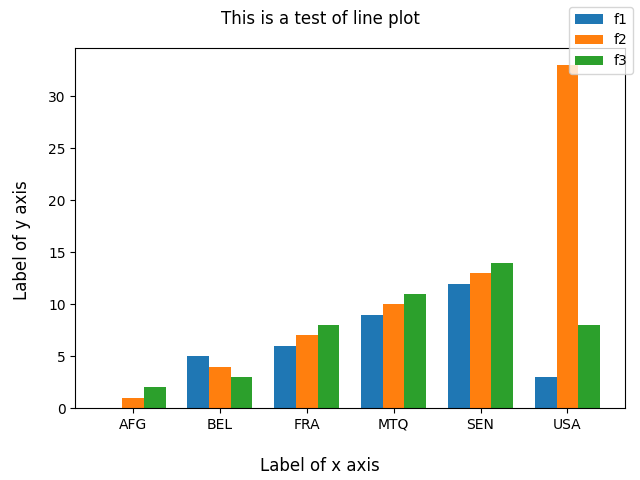
\includegraphics[scale=0.4]{../inc/graphics/histogram.png}

\end{frame}
